\chapter{Future Colliders}
\label{chapter:colliders}

\epigraph{Progress is not a straight line.}{An Wang}

In the post-LHC era, particle physics is at somewhat of an impasse. \acrfull{SM} has held up to most experiments and observation, and its predictive power is now exhausted. There are tantalising hints at a theory beyond the Standard Model -- in the form of CP-violation and dark matter -- but as of yet all new ways to probe the \acrshort{SM} for its weaknesses, to see the greater theory behind it, have yielded very little. 

There are many planned investigations to attempt to identify physics \acrlong{BSM} that use the \acrfull{LHC}, or plan to leverage the upgrades for the \acrfull{HL-LHC}. However, now that the Higgs boson has been identified successfully, one of the most fruitful avenues for further research is the construction and operation of a lepton collider at the energy frontier, with sufficient centre-of-mass energy to produce Higgs bosons in large numbers.

This is what motivates the several proposals for future lepton colliders around the world today, that would operate to complement and expand the reach of particle physicists beyond what the \acrshort{LHC} is currently capable of. These proposed lepton colliders are broadly split into two groups: linear colliders and circular colliders. 

Linear colliders use two accelerator arms pointed towards a single interaction point, and in general are capable of high centre-of-mass energies thanks to developments in accelerator technologies. The main candidates for this style of collider are the \acrfull{ILC} and the \acrfull{CLIC}. 

Circular colliders use a similar layout to the \acrshort{LHC}, with a circular accelerator capable of creating collisions at multiple different interaction points around the circumference of the ring, which permits multiple detectors. The downsides of a circular collider are that lighter particles like electrons are more prone to energy losses via synchrotron radiation, limiting the centre-of-mass energies that a circular lepton collider can operate at. However, in exchange they tend to have much higher luminosities, allowing greater numbers of collisions and higher yields of certain processes or channels. The main candidates for circular colliders are the \acrfull{FCC} and the \acrfull{CEPC}. 

These proposed colliders share many of the same motivations, design considerations, features, and challenges, as does the ongoing international effort in research and development to make these colliders a reality.

\section{The physics case for a lepton collider}
With the observation of a Higgs boson with a mass of 125 GeV, based on data from the \acrlong{LHC}, the Standard Model of particle physics is now functionally complete. All of it's major predictions have been observed. This is a testament to it's quality as a theory, where it's predictive power and accuracy is one of the best in all of the sciences.

But despite this, a multitude of observations have shown that the Standard Model cannot be a complete theory of nature. Many phenomena have been observed that the Standard Model cannot predict, or do not interact with the Standard Model in any way. In the post-LHC era, particle physics is now forced to seek answers to three questions that the Standard Model cannot provide answers to:

\begin{itemize}
	\item What is dark matter? Astrophysics observations support the existence of a neutral, weakly-interacting substance that composes around 85\% of all mass in the universe. Yet this substance cannot be explained by any known form of matter, and is completely unprecedented by the Standard Model.
	\item Why is there so little antimatter? The symmetries inherent in the Standard Model predict that the Big Bang would have created an equal quantity of matter and antimatter. Yet the universe today is dominated by matter.
	\item Why does the Higgs field fill space and give mass to elementary particles? The existence of the Higgs field and the coupling of the Higgs boson to other particles can be understood from the Standard Model but their origin or cause is still unexplained.
\end{itemize}

In order to answer these questions, new theories of physics Beyond the Standard Model (\acrshort{BSM}) have been made, and need to be experimentally tested. To do this, particle collider experiments at the energy frontier are needed. The \acrfull{LHC} has already been used extensively for searches for new particles, rare and exotic decays, supersymmetry and dark matter.

However, the running of a lepton collider at the energy frontier would be complementary to the \acrshort{LHC}'s continuing physics programme -- there are many events or channels that are inaccessible or difficult to examine in one environment that are much simpler or higher precision in the other. In this way, a lepton collider would help to improve and refine measurements already taken at the \acrshort{LHC}, while also allowing physicists to examine new channels and decays that were not accessible to it. 

This follows a historical pattern in particle physics -- as the energy frontier advances, hadron colliders are used to discover new physics and new phenomena, followed by lepton colliders to examine these phenomena in higher precision.

\subsection{Higgs physics}
Of specific interest to searches at lepton colliders would be the Higgs boson itself. Many \acrshort{BSM} models predict differences from the Standard Model in the Higgs sector -- such as several Higgs bosons with different masses, composite Higgs, charged Higgs etc. The comparatively `quiet' environment of a lepton collider allows higher precision measurements of the properties of the Higgs boson, placing better constraints on the presence of new physics. In addition, lepton colliders can easily operate at specific thresholds and ``hot spots'' for Higgs production, permitting a much greater number of events yielding Higgs bosons, and thus a greater sample to examine.

% First confirmation of h->bb decays paper: https://atlas.web.cern.ch/Atlas/GROUPS/PHYSICS/CONFNOTES/ATLAS-CONF-2018-036/
Additionally, the most common decay of the Higgs boson, at a branching ratio of 57.7\%, is the $H \rightarrow b \overline{b}$ process. Despite the high branching ratio, the huge \acrshort{QCD} backgrounds in a hadron collider have made this decay incredibly difficult to observe at the LHC -- in fact, the $H \rightarrow b \overline{b}$ decay has only fairly recently been experimentally verified by the \acrshort{ATLAS} experiment. However, in a lepton collider these \acrshort{QCD} backgrounds are significantly smaller, meaning this decay channel is much easier to analyse, opening up a huge number of Higgs events for analysis and examination.

Another highly interesting process uniquely accessible to lepton colliders is the higgstrahulung reaction: $e^+ e^- \rightarrow Zh$. The decay of the Z boson into lepton pairs $e^+ e^-$ or $\mu^+ \mu^-$ allows high precision kinematic measurements of the process without directly measuring the Higgs boson itself. This allows unprecedented measurement of the Higgs mass, while also making measurements of missing energy possible. If the Higgs boson has invisible decays -- such as dark matter particles or other undiscovered particles that don't couple to the \acrshort{SM} -- the higgstrahlung process allows their existence to be identified.

% High precision and model-independent measurement of $\Gamma\textsubscript{h}$ (total rate of Higgs decay)

\subsection{Top physics}
[...]

%=	=	=
%-Detailed study of the top quark, which is easier to reconstruct, since the LHC has such high QCD backgrounds
%-Study of top quark at threshold is difficult in hadron colliders, as the parton-parton collision has poorly define centre of mass energy
%-tt production threshold studies, which are "idealised" studies of QCD systems like the tt bound state
%-Top-Higgs Yukawa coupling is highly sensitive to new physics, since it's the strongest coupling of the Higgs
%-In many models, additional particles are partners of the top, so predict divergent top properties (includes supersymmetry, and extra dimension models)
%-The normal pattern is hadron colliders discover new quarks, and a lepton collider examines them in detail. This was true of the charm and bottom, but the top quark has not had an equivalent lepton collider (production threshold is 350 GeV, so there's been no lepton colliders at this energy range)
%=	=	=
%In general, the centre of mass energy of circular colliders is limited by losses to due synchrotron radiation. The energy loss per turn scales with $\frac{E^4}{m^4}$, meaning that lighter particles like electrons suffer more losses due to synchrotron radiation than heavier particles like hadrons. However, circular colliders provide significantly higher luminosities at energies in the 90-250 GeV range when compared to linear colliders. 
%=	=	=
% From p2, https://arxiv.org/pdf/1506.05992.pdf
% "The LHC gives access to high energies for direct production of new particles. However, this comes at a price. The rates of production of proposed new particles are typically 10−10 − 10−12 of the proton-proton total cross section. Even after selection of characteristic event types, these processes typically represent only about 10% of the total yield, over a background consisting of complex Standard Model reactions. This limits both the range of new processes that can be observed and the precision with which rates can be measured."
%=	=	=

\begin{table}[h]
\centering
	\begin{tabular}{ c | c | c }
	\hline \hline
	\textbf{Energy} & \textbf{Reaction} & \textbf{Physics goal} \\ \hline
	 91 GeV & $e^+ e^- \rightarrow Z$ & ultra-precision electroweak \\ \hline
	 160 GeV & $e^+ e^- \rightarrow WW$ & ultra-precision W mass \\ \hline
	 250 GeV & $e^+ e^- \rightarrow Zh$ & precision Higgs coupling \\ \hline
	 350-500 GeV & $e^+ e^- \rightarrow t\overline{t}$ & top quark mass and couplings \\
	   & $e^+ e^- \rightarrow WW$ & precision W coupling \\
	   & $e^+ e^- \rightarrow \nu \overline{\nu} h$ & precision Higgs coupling \\ \hline
	 500 GeV & $e^+ e^- \rightarrow f \overline{f}$ & precision search for $Z^\prime$ \\
	   & $e^+ e^- \rightarrow t \overline{t}h$ & Higgs coupling to top \\
	   & $e^+ e^- \rightarrow Zhh$ & Higgs self-coupling \\
	   & $e^+ e^- \rightarrow \widetilde{\chi} \widetilde{\chi}$ & search for supersymmetry \\
	   & $e^+ e^- \rightarrow AH, H^+, H^-$ & search for extended Higgs states \\ \hline
	 700-1000 GeV & $e^+ e^- \rightarrow \nu \overline{\nu} hh$ & Higgs self-coupling \\
	   & $e^+ e^- \rightarrow \nu \overline{\nu} VV$ & composite Higgs sector \\
	   & $e^+ e^- \rightarrow  \nu \overline{\nu} t \overline{t}$ & composite Higgs and top \\
	   & $e^+ e^- \rightarrow \tilde{t} \tilde{t}^*$ & search for supersymmetry \\ \hline
	\end{tabular}
	\caption{Physics processes of interest at lepton colliders up to 1 TeV.}
	\label{table:colliders/physics-goals}
\end{table}

[...]

\section{The International Linear Collider}
The \acrfull{ILC} is a proposed high-luminosity linear electron-positron collider based upon 1.3GHz superconducting radio frequency (SCRF) accelerating technology. The centre of mass energy ($\sqrt{s}$) would be 250 GeV, upgradable to 500 GeV and then to 1 TeV at a later date. The total footprint of the complex would be 31km in length, with the arms using magnets with an accelerating gradient of 31.5 MVm\^{-1} in metre-long superconducting nine-cell niobium cavities operating at 2K.

The ILC is also planned to operate on an innovative ``push-pull'' system of detectors -- two detectors are planned, called the \acrfull{ILD} and \acrfull{SiD}, which would be mounted on a movable base. The detector hall would be large enough to accommodate both detectors such that they could be interchanged.

There were a number of proposed sites for the ILC, including CERN in Geneva, DESY in Hamburg, and \acrshort{JINR} near Moscow. The most recent country to seek to host the collider was Japan, who proposed a greenfield site located in the Kitakami Highlands region of Iwate prefecture. 

However, a report from the Science Council of Japan (a representative organisation of the Japanese science community) released in early 2019 expressed that they had not reached a consensus as to whether to support hosting the ILC in Japan. Some  of the reasons cited were concerns over international cost-sharing in the long-term, as well as whether the expected scientific outcomes would justify the unprecedented human resource requirements and infrastructure necessary to make the ILC a reality \cite{linearcolliders-scj-report}.

%Reference (24/04/2019): http://www.linearcollider.org/content/decision-international-linear-collider-“not-what-we-had-hoped-progress-nevertheless” 
On 7th March 2019, the Japanese government expressed that it would not make a proposal to host the collider in Japan. The Japanese government did however express interest in the ILC, and declared that it would be continuing discussion and interest in the project as a whole.

%-Beam polarisation allows a high rate of higgstrahlung processes, and thus a high number of Higgs events to examine


[...]

\subsection{The ILD and SiD detectors}
[...]

One of the unique features of the ILC is the push-pull detector system. This is a moving platform in the chamber housing the interaction point, upon which two detectors can be mounted. The platform can be moved to change which detector is in the beamline, allowing a linear collider to function with multiple detectors. Switching detectors is expected to take [some] hours. This allows the two detectors to specialise for different physics studies and goals, much like the experiments at the Large Hadron Collider at CERN, which is normally not possible with linear colliders. [?] [...]

\subsubsection{The International Large Detector (ILD)}
[...]

The finished ILD will weigh 14,000 metric tonnes, and using a magnetic field of 3.5 Tesla will offer a spatial resolution of 3 microns in the vertex tracker, and 60 microns in the central TPC tracker. 

\begin{figure}[h]
	\centering
	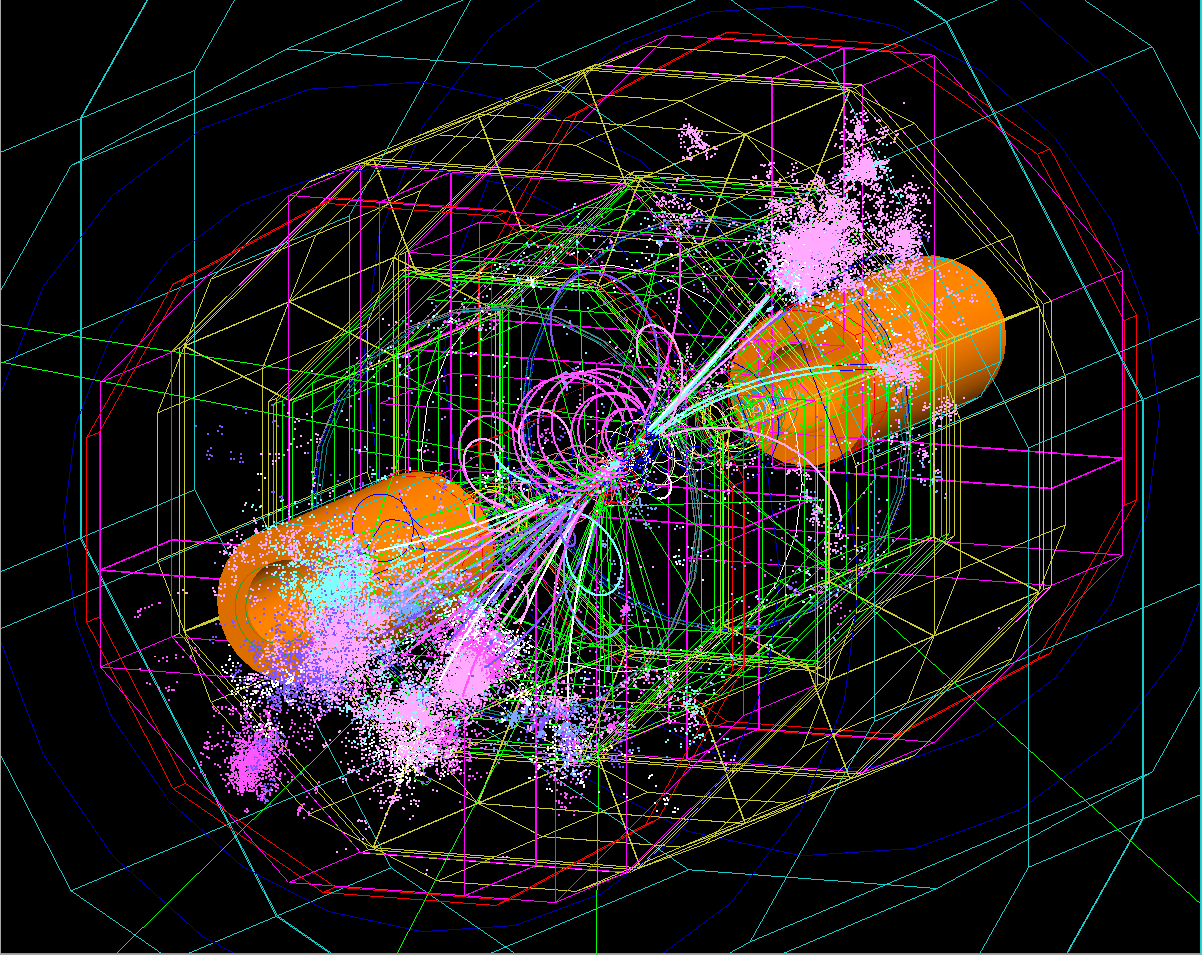
\includegraphics[width=0.75\textwidth]{../Pictures/SimulatedEvent1.png}
	\caption{Visualisation of a simulated tth event in the ILD. Charged particles can be easily identified by their curved, coiled or spiral paths, and the jets are clearly visible as the light pink and purple areas near the beampipes on either side.}
	\label{figure:colliders/ILD/tth-simulation}
\end{figure}

\subsubsection{The Silicon Detector (SiD)}
[...]

\section{The Compact Linear Collider}
[...]

The CLIC project foresees a programme spanning 22 years, over which multiple upgrades to the centre-of-mass energy would take place. Initial construction would be at 380 GeV, focusing on precision measurements of top-quark and Higgs physics. Further upgrades would increase the centre-of-mass energy to 1.5 TeV, then finally 3 GeV. Physics goals in these later stages would involve searches for new physics processes, as well as precision measurements of rare Higgs processes, and of new states discovered at the LHC or earlier stages of CLIC. 

[...] CLIC would be built beneath the existing LHC ring at CERN, stretching across the French-Swiss border and running parallel to the feet of the Jura mountain range. This placement is determined by the geological features of the region around Geneva and the feet of the Juras, [...]


[...]

As of writing, the CLIC project has been submitted as input for the European Particle Physics Strategy Update, which will decide which projects the CERN collaboration chooses to pursue from 2020  onwards. [...]

CLIC's initial centre-of-mass energy will be 380 GeV, with successive upgrades increasing this to 1.5 TeV and finally 3 TeV. 

\section{The Future Circular Collider}
The \acrfull{FCC} is a series of concepts for a future collider that would be located in the Geneva area near the existing LHC ring. The FCC project as a whole has three different accelerator concepts -- the FCC-hh for proton/proton and ion/ion collisions, the FCC-ee for electron/positron collisions, and the FCC-he for electron/proton collisions.

The initial proposal is to construct a circular electron/positron collider -- the FCC-ee -- with a circumference of 100km and delivering a maximum centre-of-mass energy of 365 GeV. The motivation for this is that at this energy range -- the electroweak scale -- the FCC would be able to access the Z pole, the W- and top-pair production thresholds, as well as producing a large number of Higgs bosons. 

A further part of the proposal for the FCC is that following the conclusion of the physics programme of the FCC-ee, the tunnels constructed to house the accelerator would be re-used for the FCC-hh, a hadron collider. This follows a similar use case as the LHC, which re-purposed the tunnels used for the \acrfull{LEP}. It is claimed that the FCC-hh built in these tunnels would be able to reach centre-of-mass energies of at least 100 TeV.

According to the given timeline, the FCC-ee would begin construction in 2028, and first physics would take place in 2039. 

%FCC-ee physics:
%-Much higher luminosity beneath 400GeV
%-Multiple interaction points
%-Precision beam energy measurement through resonant transverse depolarisation
%-(Linear colliders have higher energy, easier longitudinal beam polarisation)
%-Large Higgs samples allows study of flavour-violating Higgs and very rare SM decays

[...]

\section{The Circular Electron Positron Collider}

The \acrfull{CEPC} is a proposal for a circular electron-positron collider 

[...]